\documentclass{standalone}
\usepackage{tikz}
\usetikzlibrary{patterns, positioning}

\begin{document}
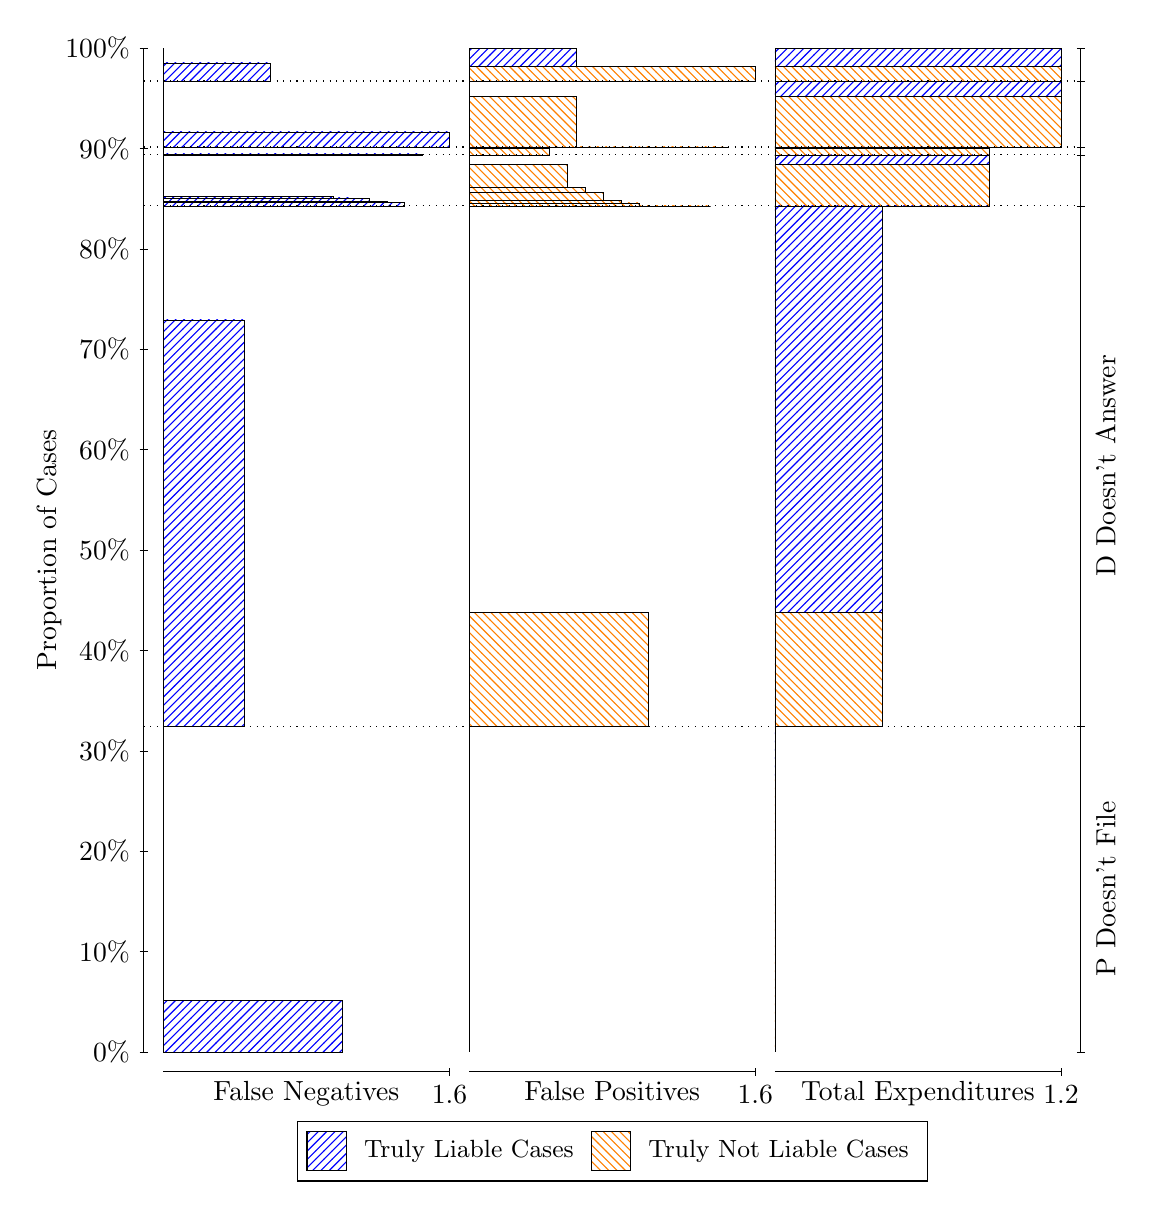
\begin{tikzpicture}
\draw[black, very thin] (1.5,1.75) -- (1.5,14.5);
\node[rotate=90, anchor=center] at (0.3, 8.125) {Proportion of Cases};
\draw[black, very thin] (1.45,1.75) -- (1.55,1.75);
\node[anchor=east] at (1.45, 1.75) {0\%};
\draw[black, very thin] (1.45,3.025) -- (1.55,3.025);
\node[anchor=east] at (1.45, 3.025) {10\%};
\draw[black, very thin] (1.45,4.3) -- (1.55,4.3);
\node[anchor=east] at (1.45, 4.3) {20\%};
\draw[black, very thin] (1.45,5.575) -- (1.55,5.575);
\node[anchor=east] at (1.45, 5.575) {30\%};
\draw[black, very thin] (1.45,6.85) -- (1.55,6.85);
\node[anchor=east] at (1.45, 6.85) {40\%};
\draw[black, very thin] (1.45,8.125) -- (1.55,8.125);
\node[anchor=east] at (1.45, 8.125) {50\%};
\draw[black, very thin] (1.45,9.4) -- (1.55,9.4);
\node[anchor=east] at (1.45, 9.4) {60\%};
\draw[black, very thin] (1.45,10.675) -- (1.55,10.675);
\node[anchor=east] at (1.45, 10.675) {70\%};
\draw[black, very thin] (1.45,11.95) -- (1.55,11.95);
\node[anchor=east] at (1.45, 11.95) {80\%};
\draw[black, very thin] (1.45,13.225) -- (1.55,13.225);
\node[anchor=east] at (1.45, 13.225) {90\%};
\draw[black, very thin] (1.45,14.5) -- (1.55,14.5);
\node[anchor=east] at (1.45, 14.5) {100\%};

\draw[black, very thin] (13.4,1.75) -- (13.4,14.5);
\draw[black, very thin] (13.35,1.75) -- (13.45,1.75);
\node[anchor=west] at (13.35, 1.75) {};
\draw[black, very thin] (13.35,5.8876) -- (13.45,5.8876);
\node[anchor=west] at (13.35, 5.8876) {};
\draw[black, very thin] (13.35,12.495) -- (13.45,12.495);
\node[anchor=west] at (13.35, 12.495) {};
\draw[black, very thin] (13.35,13.144) -- (13.45,13.144);
\node[anchor=west] at (13.35, 13.144) {};
\draw[black, very thin] (13.35,13.243) -- (13.45,13.243);
\node[anchor=west] at (13.35, 13.243) {};
\draw[black, very thin] (13.35,13.244) -- (13.45,13.244);
\node[anchor=west] at (13.35, 13.244) {};
\draw[black, very thin] (13.35,14.081) -- (13.45,14.081);
\node[anchor=west] at (13.35, 14.081) {};
\draw[black, very thin] (13.35,14.5) -- (13.45,14.5);
\node[anchor=west] at (13.35, 14.5) {};

\draw[black, very thin, pattern color=blue, pattern=north east lines] (1.75,1.75) rectangle (4.0208,2.4069);
\draw[black, very thin, pattern color=orange, pattern=north west lines] (1.75,2.4069) rectangle (1.75,5.8876);
\draw[black, very thin, pattern color=blue, pattern=north east lines] (1.75,5.8876) rectangle (2.7719,11.047);
\draw[black, very thin, pattern color=orange, pattern=north west lines] (1.75,11.047) rectangle (1.75,12.495);
\draw[black, very thin, pattern color=blue, pattern=north east lines] (1.75,12.495) rectangle (4.8156,12.535);
\draw[black, very thin, pattern color=blue, pattern=north east lines] (1.75,12.535) rectangle (4.5885,12.55);
\draw[black, very thin, pattern color=blue, pattern=north east lines] (1.75,12.55) rectangle (4.3615,12.586);
\draw[black, very thin, pattern color=blue, pattern=north east lines] (1.75,12.586) rectangle (4.1344,12.586);
\draw[black, very thin, pattern color=blue, pattern=north east lines] (1.75,12.586) rectangle (4.1344,12.598);
\draw[black, very thin, pattern color=blue, pattern=north east lines] (1.75,12.598) rectangle (3.9073,12.62);
\draw[black, very thin, pattern color=blue, pattern=north east lines] (1.75,12.62) rectangle (3.6802,12.62);
\draw[black, very thin, pattern color=blue, pattern=north east lines] (1.75,12.62) rectangle (3.4531,12.62);
\draw[black, very thin, pattern color=blue, pattern=north east lines] (1.75,12.62) rectangle (3.226,12.62);
\draw[black, very thin, pattern color=blue, pattern=north east lines] (1.75,12.62) rectangle (2.999,12.62);
\draw[black, very thin, pattern color=orange, pattern=north west lines] (1.75,12.62) rectangle (1.75,13.144);
\draw[black, very thin, pattern color=blue, pattern=north east lines] (1.75,13.144) rectangle (5.0427,13.157);
\draw[black, very thin, pattern color=orange, pattern=north west lines] (1.75,13.157) rectangle (1.75,13.243);
\draw[black, very thin, pattern color=blue, pattern=north east lines] (1.75,13.243) rectangle (2.7719,13.244);
\draw[black, very thin, pattern color=orange, pattern=north west lines] (1.75,13.244) rectangle (1.75,13.244);
\draw[black, very thin, pattern color=blue, pattern=north east lines] (1.75,13.244) rectangle (5.3833,13.435);
\draw[black, very thin, pattern color=orange, pattern=north west lines] (1.75,13.435) rectangle (1.75,14.081);
\draw[black, very thin, pattern color=blue, pattern=north east lines] (1.75,14.081) rectangle (3.1125,14.31);
\draw[black, very thin, pattern color=orange, pattern=north west lines] (1.75,14.31) rectangle (1.75,14.5);
\draw[black, very thin, pattern color=orange, pattern=north west lines] (5.6333,1.75) rectangle (5.6333,5.2307);
\draw[black, very thin, pattern color=blue, pattern=north east lines] (5.6333,5.2307) rectangle (5.6333,5.8876);
\draw[black, very thin, pattern color=orange, pattern=north west lines] (5.6333,5.8876) rectangle (7.9042,7.3363);
\draw[black, very thin, pattern color=blue, pattern=north east lines] (5.6333,7.3363) rectangle (5.6333,12.495);
\draw[black, very thin, pattern color=orange, pattern=north west lines] (5.6333,12.495) rectangle (8.699,12.495);
\draw[black, very thin, pattern color=orange, pattern=north west lines] (5.6333,12.495) rectangle (8.4719,12.495);
\draw[black, very thin, pattern color=orange, pattern=north west lines] (5.6333,12.495) rectangle (8.2448,12.495);
\draw[black, very thin, pattern color=orange, pattern=north west lines] (5.6333,12.495) rectangle (8.0177,12.496);
\draw[black, very thin, pattern color=orange, pattern=north west lines] (5.6333,12.496) rectangle (7.7906,12.533);
\draw[black, very thin, pattern color=orange, pattern=north west lines] (5.6333,12.533) rectangle (7.5635,12.562);
\draw[black, very thin, pattern color=orange, pattern=north west lines] (5.6333,12.562) rectangle (7.5635,12.563);
\draw[black, very thin, pattern color=orange, pattern=north west lines] (5.6333,12.563) rectangle (7.3365,12.664);
\draw[black, very thin, pattern color=orange, pattern=north west lines] (5.6333,12.664) rectangle (7.1094,12.732);
\draw[black, very thin, pattern color=orange, pattern=north west lines] (5.6333,12.732) rectangle (6.8823,13.019);
\draw[black, very thin, pattern color=blue, pattern=north east lines] (5.6333,13.019) rectangle (6.4281,13.019);
\draw[black, very thin, pattern color=blue, pattern=north east lines] (5.6333,13.019) rectangle (6.201,13.019);
\draw[black, very thin, pattern color=blue, pattern=north east lines] (5.6333,13.019) rectangle (5.974,13.019);
\draw[black, very thin, pattern color=blue, pattern=north east lines] (5.6333,13.019) rectangle (5.7469,13.019);
\draw[black, very thin, pattern color=blue, pattern=north east lines] (5.6333,13.019) rectangle (5.6333,13.144);
\draw[black, very thin, pattern color=orange, pattern=north west lines] (5.6333,13.144) rectangle (6.6552,13.231);
\draw[black, very thin, pattern color=blue, pattern=north east lines] (5.6333,13.231) rectangle (5.6333,13.243);
\draw[black, very thin, pattern color=orange, pattern=north west lines] (5.6333,13.243) rectangle (8.926,13.244);
\draw[black, very thin, pattern color=blue, pattern=north east lines] (5.6333,13.244) rectangle (6.6552,13.244);
\draw[black, very thin, pattern color=orange, pattern=north west lines] (5.6333,13.244) rectangle (6.9958,13.889);
\draw[black, very thin, pattern color=blue, pattern=north east lines] (5.6333,13.889) rectangle (5.6333,14.081);
\draw[black, very thin, pattern color=orange, pattern=north west lines] (5.6333,14.081) rectangle (9.2667,14.27);
\draw[black, very thin, pattern color=blue, pattern=north east lines] (5.6333,14.27) rectangle (6.9958,14.5);
\draw[black, very thin, pattern color=orange, pattern=north west lines] (9.5167,1.75) rectangle (9.5167,5.2307);
\draw[black, very thin, pattern color=blue, pattern=north east lines] (9.5167,5.2307) rectangle (9.5167,5.8876);
\draw[black, very thin, pattern color=orange, pattern=north west lines] (9.5167,5.8876) rectangle (10.879,7.3363);
\draw[black, very thin, pattern color=blue, pattern=north east lines] (9.5167,7.3363) rectangle (10.879,12.495);
\draw[black, very thin, pattern color=orange, pattern=north west lines] (9.5167,12.495) rectangle (12.242,12.495);
\draw[black, very thin, pattern color=blue, pattern=north east lines] (9.5167,12.495) rectangle (12.242,12.495);
\draw[black, very thin, pattern color=orange, pattern=north west lines] (9.5167,12.495) rectangle (12.242,13.019);
\draw[black, very thin, pattern color=blue, pattern=north east lines] (9.5167,13.019) rectangle (12.242,13.144);
\draw[black, very thin, pattern color=orange, pattern=north west lines] (9.5167,13.144) rectangle (12.242,13.144);
\draw[black, very thin, pattern color=blue, pattern=north east lines] (9.5167,13.144) rectangle (12.242,13.144);
\draw[black, very thin, pattern color=orange, pattern=north west lines] (9.5167,13.144) rectangle (12.242,13.231);
\draw[black, very thin, pattern color=blue, pattern=north east lines] (9.5167,13.231) rectangle (12.242,13.243);
\draw[black, very thin, pattern color=orange, pattern=north west lines] (9.5167,13.243) rectangle (12.242,13.244);
\draw[black, very thin, pattern color=blue, pattern=north east lines] (9.5167,13.244) rectangle (12.242,13.244);
\draw[black, very thin, pattern color=orange, pattern=north west lines] (9.5167,13.244) rectangle (13.15,13.889);
\draw[black, very thin, pattern color=blue, pattern=north east lines] (9.5167,13.889) rectangle (13.15,14.081);
\draw[black, very thin, pattern color=orange, pattern=north west lines] (9.5167,14.081) rectangle (13.15,14.27);
\draw[black, very thin, pattern color=blue, pattern=north east lines] (9.5167,14.27) rectangle (13.15,14.5);
\draw[black, dotted] (1.5,5.8876) -- (13.4,5.8876);
\draw[black, dotted] (1.5,12.495) -- (13.4,12.495);
\draw[black, dotted] (1.5,13.144) -- (13.4,13.144);
\draw[black, dotted] (1.5,13.243) -- (13.4,13.243);
\draw[black, dotted] (1.5,13.244) -- (13.4,13.244);
\draw[black, dotted] (1.5,14.081) -- (13.4,14.081);
\draw[black, very thin] (1.75,1.5) -- (5.3833,1.5);
\node[anchor=north] at (3.5667, 1.5) {False Negatives};
\draw[black, very thin] (5.3833,1.45) -- (5.3833,1.55);
\node[anchor=north] at (5.3833, 1.45) {1.6};

\draw[black, very thin] (5.6333,1.5) -- (9.2667,1.5);
\node[anchor=north] at (7.45, 1.5) {False Positives};
\draw[black, very thin] (9.2667,1.45) -- (9.2667,1.55);
\node[anchor=north] at (9.2667, 1.45) {1.6};

\draw[black, very thin] (9.5167,1.5) -- (13.15,1.5);
\node[anchor=north] at (11.333, 1.5) {Total Expenditures};
\draw[black, very thin] (13.15,1.45) -- (13.15,1.55);
\node[anchor=north] at (13.15, 1.45) {1.2};

\node[black, centered, rotate=90] at (13.72, 3.8188) {P Doesn't File};
\node[black, centered, rotate=90] at (13.72, 9.1914) {D Doesn't Answer};






\draw (7.449999999999999,1.5) node[draw=none] (baseCoordinate) {};
\begin{scope}[align=center]
        \matrix[scale=0.5, draw=black, below=0.5cm of baseCoordinate, nodes={draw}, column sep=0.1cm]{
            \node[rectangle, draw, minimum width=0.5cm, minimum height=0.5cm, pattern=north east lines, pattern color=blue] {}; &
            \node[draw=none, font=\small] (B) {Truly Liable Cases}; &
            \node[rectangle, draw, minimum width=0.5cm, minimum height=0.5cm, pattern=north west lines, pattern color=orange] {}; &
            \node[draw=none, font=\small] (B) {Truly Not Liable Cases}; \\
            };
\end{scope}

\end{tikzpicture}
\end{document}